
\section{\centering FIELD ORIENTED CONTROL}

\subsection{INTRODUCTION}

\hspace{0.2in}The FOC control loop shown involves some key mathematical transformations like the Clarke and Park transforms. The 3-phase stator currents are transformed to a 2-phase orthogonal reference frame by the Clarke transform. The Park transform then rotates this into the synchronous rotational reference frame aligned with the rotor flux. The required rotor position is obtained using incremental encoders, Hall-effect sensors, or sensorless methods. The flux and torque components in this rotating reference frame are decoupled, allowing for separate control through the PI controllers. The outputs of the PI controllers are transformed back to 3-phase voltages to drive the inverter. Space vector PWM is typically used to generate the gate signals for the inverter.
\subsection{BLOCK DIAGRAM OF FIELD ORIENTED CONTROL}

\hspace{0.2in}The Field Oriented Control (FOC) block diagram depicts the implementation of vector control of an AC induction motor (ACIM) using MATLAB. The desired speed ($\omega_{\text{ref}}$) is fed into a Proportional-Integral (PI) speed controller to compute the torque reference ($T_{\text{ref}}$). This torque reference, in conjunction with the ACIM control reference, is used to determine the reference direct and quadrature axis currents ($I_{sd_{\text{ref}}}$ and $I_{sq_{\text{ref}}}$), managed by two separate PI controllers for current regulation. The Park transform takes actual motor currents ($I_a, I_b$) and transforms them using the rotor's electrical position ($\theta_e$), obtained from a position generator along with a sine-cosine lookup. The Inverse Park transform takes the PI controllers' output ($V_{sd_{\text{ref}}}$ and $V_{sq_{\text{ref}}}$) and converts them back to the stationary reference frame ($V_{\alpha}$, $V_{\beta}$). Subsequently, these voltages are fed to a space vector generator that produces pulse-width modulation (PWM) signals for the inverter, which then drives the induction motor. The motor's actual speed ($\omega_r$) is measured and compared to the reference speed to ensure closed-loop control. Additionally, the slip speed estimator feeds into the position generator for accurate control, completing the FOC system loop. The block diagram shown in Fig. \ref{fig:FOCblock} depicts the main components of FOC for induction motor drive.


\begin{figure}
\centering
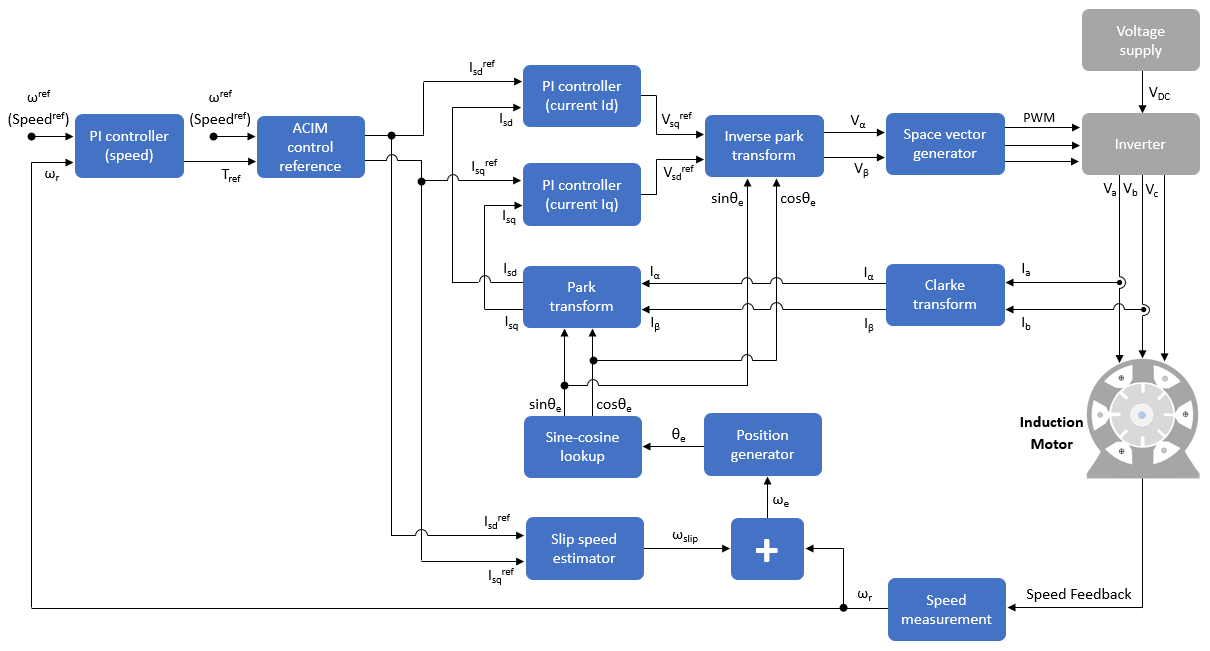
\includegraphics[width=1.2\textwidth]{sections/section2/images/blockDiagram.png}
\caption{Block Diagram Of FOC For I.M.}
\label{fig:FOCblock}
\end{figure}



This block diagram represents a typical vector control (also known as field-oriented control) for an AC Induction Motor (ACIM). It's an advanced control strategy used in variable frequency drives (VFDs) to control the torque and speed of a three-phase AC induction motor. Let's discuss each block and their roles in the control scheme:

\begin{enumerate}


  \item {PI Controller (speed):} This is a Proportional-Integral controller for the speed loop. It takes the speed reference ($\omega_{\text{ref}}$ or Speed\textsuperscript{ref}) and compares it with the actual rotor speed ($\omega_r$). The output of the PI controller is a reference torque ($T_{\text{ref}}$), which sets the desired motor torque corresponding to the target speed.
  
  \item {ACIM Control Reference:} It translates the reference torque into current components that will achieve this torque. These current components are referenced in the d-q coordinate system, where $I_{sd}^{\text{ref}}$ is the direct-axis current reference, and $I_{sq}^{\text{ref}}$ is the quadrature-axis current reference.
  
  \item {PI Controllers (current $I_d$ and $I_q$):} There are two PI controllers here for the current loop---one for the direct-axis current ($I_{sd}$) and another for the quadrature-axis current ($I_{sq}$). These controllers ensure that actual motor currents match the current references derived from the speed controller.
  
  \item {Park Transform:} This block transforms the three-phase stator currents ($I_a$, $I_b$, $I_c$) into a two-axis current vector ($I_d$, $I_q$) in the rotating reference frame (d-q frame), which simplifies control of the motor.
  
  \item {Sine-cosine Lookup and Position Generator:} It provides the sine and cosine of the electrical angle $\theta_e$, which is required for the Park and inverse Park transforms. The position generator computes the rotor's electrical angle based on the rotor speed and slip frequency, which is the difference between the electrical frequency and the mechanical rotor speed frequency.
  
  \item {Slip Speed Estimator:} It estimates the slip speed ($\omega_{\text{slip}}$) of the motor, which is the difference between the synchronous speed and the actual rotor speed. This is used, along with the rotor speed, to compute the electrical angle.
  
  \item {Inverse Park Transform:} This block takes the current references in the d-q axis ($V_{sd}^{\text{ref}}$, $V_{sq}^{\text{ref}}$) and converts them into voltage references in the stationary reference frame ($V_\alpha$, $V_\beta$) required for generating PWM signals.
  
  \item {Space Vector Generator:} This module generates the PWM (Pulse Width Modulation) signals necessary to control switches in the  
   inverter, based on the stationary reference frame voltages.
  
  \item {Inverter:} The inverter takes the DC voltage supply ($V_{dc}$) and switches it to synthesize variable-frequency AC voltage for the motor using the PWM signals it receives. This results in three-phase output voltages ($V_a$, $V_b$, $V_c$) that control the motor.
  
  \item {Induction Motor:} The actual physical motor that converts electrical power into mechanical power, which is controlled by the variable input voltages.
  
  \item {Clarke Transform:} This converts the three-phase stator currents ($I_a$, $I_b$, $I_c$) into two orthogonal components ($I_\alpha$, $I_\beta$) in the stationary reference frame, which is a precursor for the Park transform.
  
  \item {Speed Feedback:} The rotor speed is measured and fed back into the control system to adjust the control signal and maintain the desired speed accurately.
\end{enumerate}





\subsection{WORKING OF FOC}
The main components and their working is as follows:

\begin{enumerate}
    
\item Three phase voltages and currents from the motor are converted to two phase stationary reference frame using Clarke transformation.

\item The stationary reference frame is then converted to synchronous rotating reference frame aligned with the rotor flux using Park transformation.

\item Using feedback of rotor position/speed, flux and torque controllers generate reference current components in rotating frame.

\item Inverse Park and Clarke transforms convert these reference currents to three phase currents for the voltage source inverter.

\item SVPWM scheme is used to generate switching pulses for the inverter to achieve the reference currents.

\item Inverter supplies controlled three phase voltages to drive the induction motor.

\item Rotor position/speed sensor provides feedback for transformation calculations.
\end{enumerate}

\subsection{CHAPTER SUMMARY}
\hspace{0.2in} Introduction, block diagram and working of FOC are presented in this chapter.

\newpage